\chapter{R�ALISATION}

%\begin{abstract}
\section{Introduction}
	We design a complete codec system using a feed forward neural network. The model is being trained the autoencoder while each number in the code has been rounded up to the closest centroid.
%\end{abstract}

\section{Introduction and Background}
Codecs are algorithms consist of two parts, encoder and decoder. The Encoder transforms the information signal (audio, video, image, etc.) to a bit stream. The decoder map the bit stream to the original signal space. The main challenge in designing a codec is to keep the quality while remaining the bit rate low.\\
In this work the codec is being designed by learning the weight of a feed forward neural network. 
We simplify the the codec by the autoencoder associated with a vector quantizer.\\
Autoencoders are multi-layer feed forward neural networks which are used to initialize to the neural nets for other (like classification, etc.) tasks. Generally autoencoders use weight sharing techniques to reduce the complexity and number of parameters, i.e. the networks is divided to the symmetric sub networks. Weight matrix are transpose of each other in corresponding layers. We call the second half of the network \textit{decoder} and the first half followed by a vector quantizer system the \textit{encoder}.\\
Vector quantizer is a algorithm seeking for centroids as density points of nearby lying samples and represent each point by its closest centroid. The set of all centroids is known as \textit{code-book}. The code-book can be constructed by k-means algorithm and its cardinality is a pre-determined parameter in this model. See Figure \ref{fig:autoencoder}). Similar ideas have been visited in \cite{atreya} in general and in \cite{deng} for spectrogram of the audio signal.

\begin{figure}[h]
	\centering
	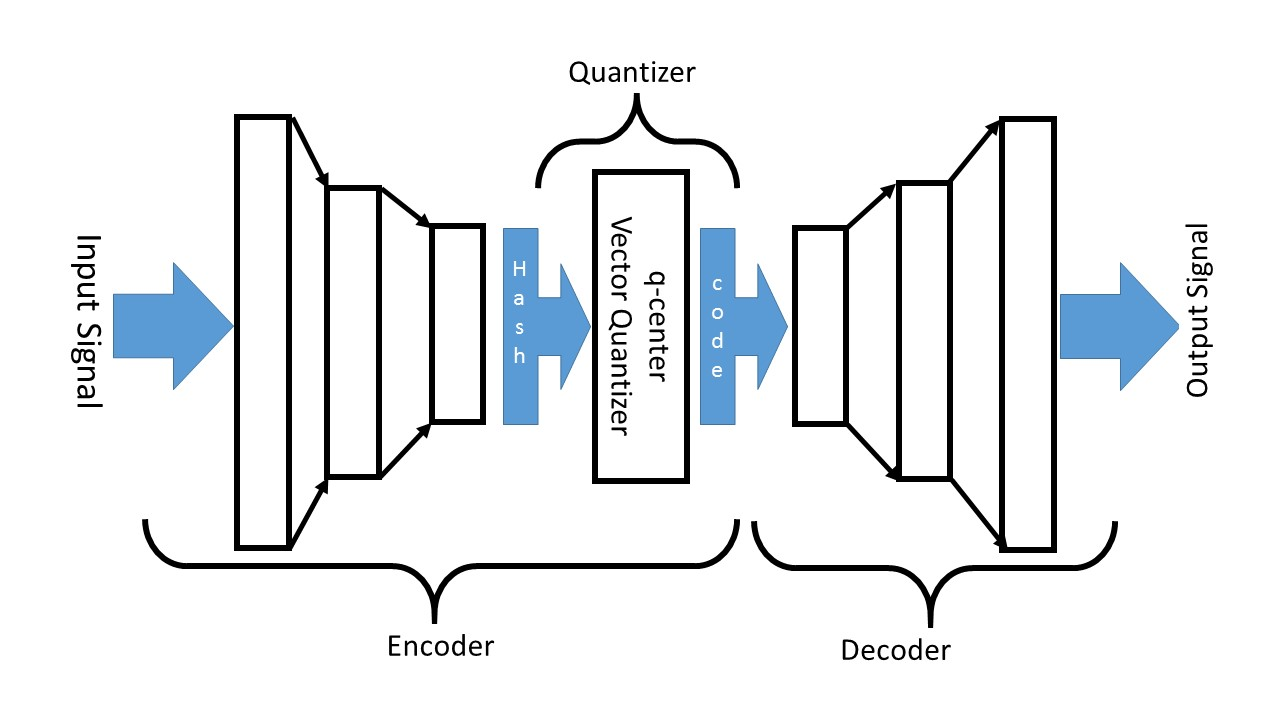
\includegraphics[width=1.2\textwidth]{AutoEncoder_2.jpg}
	\caption{Block diagram of the Codec based on stacked autoencoders \label{fig:autoencoder}}
\end{figure} 

\section{Experiments}
We run the experiment on the "mnist" dataset.  $60000$ samples in form of vectors, size $784 \times 1$. The data has been normalized between $0$ and $1$ beforehand.\\
We conduct different experiments by changing the number of layers and number of units in each layer. We kept the number of neurons just before and after vector quantization layer the constant number of $256$ units. The transfer function fixed to \textit{sigmoid}, $y = \frac{1}{1 + e^{-x}}$ for all the layers. 
the hidden layers in different experiments posses variant values of the set $ \{ 128, 256, 512, 1024\}$ and number of hidden layers varies from $2$ to $4$ in different experiments.\\
At the beginning of every epoch, Vector quantization algorithm finds $q$ centroids among the outputs of the encoder (hash vectors) and replace each hash vector element by its corresponding (closest) centroid in the code-book.\\
The objective function is the Euclidean distance between the input and the output signal (waveform matching approach). The training has been done using backpropagation algorithm. We have used Optimizer that implements the Adam algorithm. It is a gradient-based optimization based on adaptive estimation of moments. This algorithm does not perform worst than the other competitors.
\section{Results}
The main parameter we sweep over and monitor the results is the effect of the number of centroids over the Signal to Noise Ratio (snr) which calculated based on $l^2$ distance between the original signal and the reconstructed signal.
As we expected, generally snr will increase with more centroid, the snr improvement rate is proportional to inverse of the number of centroids. See Figures \ref{fig:SNR1} and \ref{fig:SNR2}. \\

The main distortion caused by the coding system and the quantization mechanism is visible as blurred edges and some low power confusions on the smooth areas of the image.See Figures \ref{fig:SNR1} and \ref{fig:SNR2}.\\
The behavior of snr curve remains quit similar in different  trials. We conducted various experiments on a variety of network parameters. These parameters consist of basic structure defining parameters like number of hidden layers and number of units per each layer and training parameters like batch size, learning rate, and maximum epoch.

\begin{figure}[!]
	\centering
	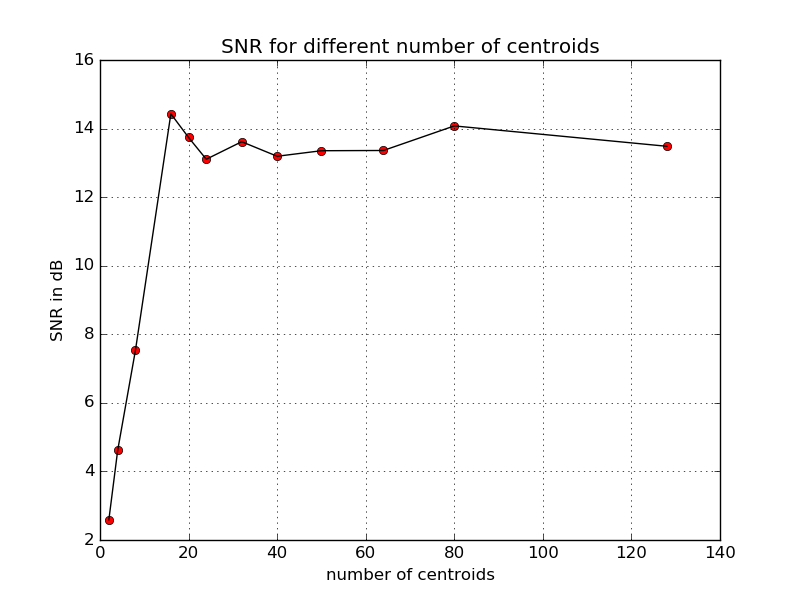
\includegraphics[width=1\textwidth]{v-recons.png}
	\caption{SNR different number of centroids  for network \{1024, 512, 256 \} \label{fig:SNR1}}
\end{figure} 

\begin{figure}[h]
	\centering
	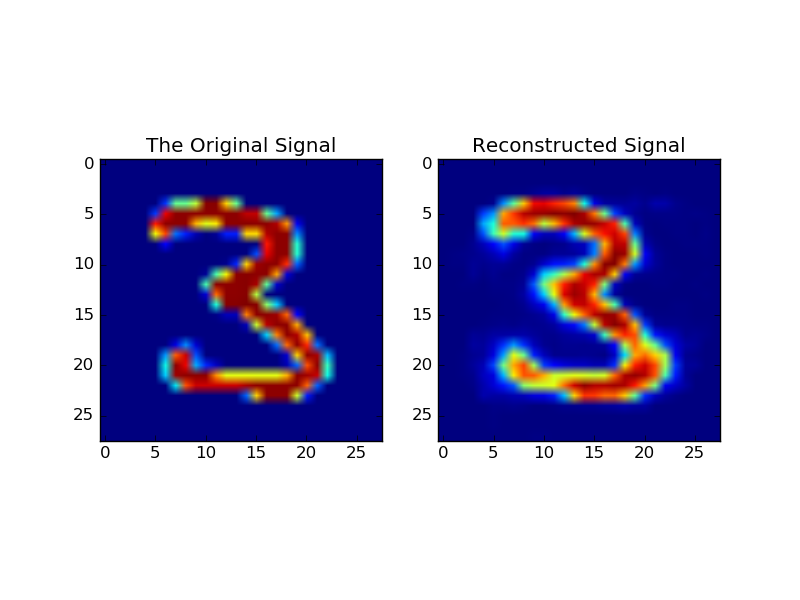
\includegraphics[width=1.\textwidth]{2v-recons-9.png}
	\caption{A sample Input and output of the network\{512, 1024,256 \} and 20 centroids \label{fig:sample1}}
\end{figure}

\begin{figure}[hb]
	\centering
	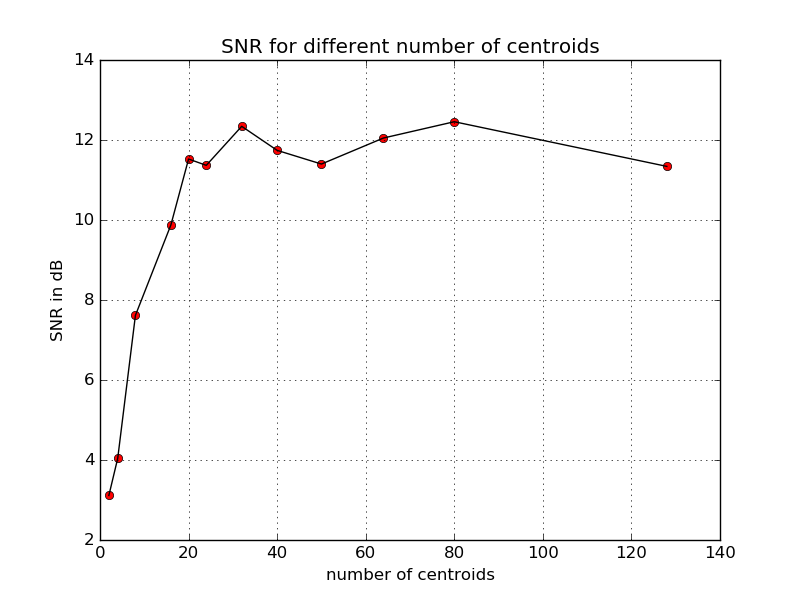
\includegraphics[width=1\textwidth]{v-recons2.png}
	\caption{SNR different number of centroids  for network \{512, 1024,256 \} \label{fig:SNR2}}
\end{figure}

\section{Discussion}
The similarity of snr curves and its saturation behavior for large number of  centroids is can be result of several causes. We hypothesize that this saturation may reflect the learning capacity of this network with that particular learning algorithm. The other hypothesis states that this estimator is biased and there will be some level of distortion on reconstruction for this input signal given the quantized observations.
\section{Future works}
We will examine different network structure (deeper networks), different units (convolutional, LSTM, etc.), different training algorithm and its effect on the performance of the model, and coding ability of this model for different data modulities such as audio in transform domain and time domain. Prove or reject of the hypothesis provided in section before is also the question of interest from theoretical view point.


\begin{thebibliography}{99}
	\bibitem{atreya2009novel} 
	Atreya, Anand and O?Shea, Daniel. 
	\textit{Novel Lossy Compression Algorithms with Stacked Autoencoders}. 
	
	\bibitem{deng}
	Deng, Li and Seltzer, Michael L and Yu, Dong and Acero, Alex and Mohamed, Abdel-Rahman and Hinton, Geoffrey E.
	\textit{Binary coding of speech spectrograms using a deep auto-encoder}.
	Interspeech,1692-1695,2010,Citeseer.
\end{thebibliography}